\section{DRAM}

\textbf{Memory-Access Protocol}

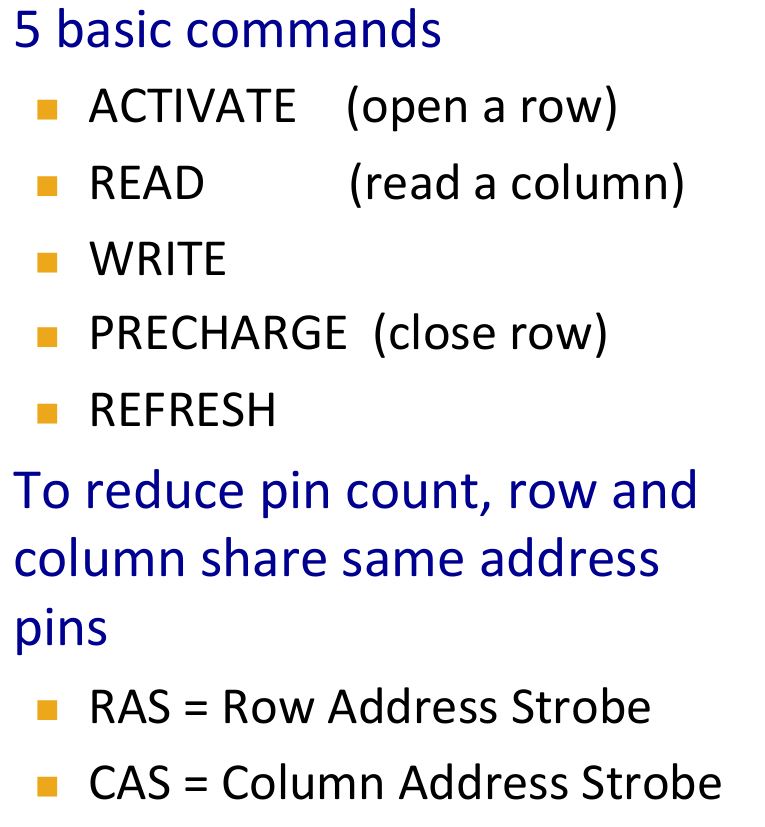
\includegraphics[width=\linewidth]{png/dram.png}

Modern DRAM chips consist of multiple banks, they operate independently, but
share command/address/data pins, each bank can have a different row active so we
can overlabp ACTIVATE and PRECHARGE latencies, e.g. READ to bank 0 while ACTIVATING bank 1

\textbf{DRAM High Level}

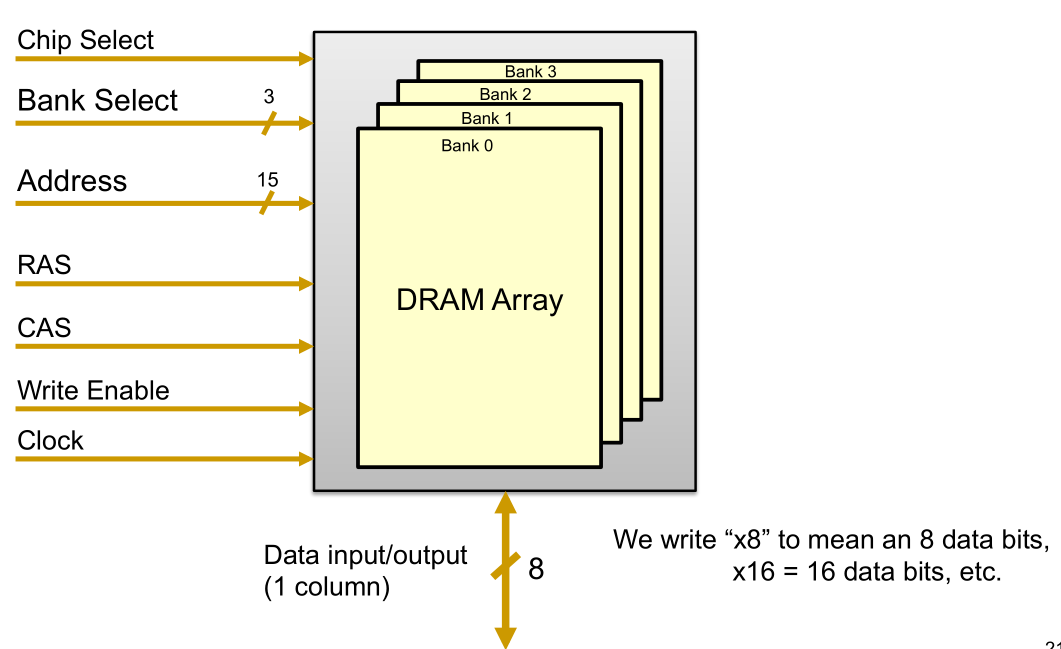
\includegraphics[width=\linewidth]{png/drambank.png}

\textbf{Ranks} A 64-bit DIMM with 16 chips with x8 interfaces has 2 ranks, each
64-bit group of chips is called a rank, all chips in a rank respond to the same
command

\textbf{DRAM Channels} All DIMMs get the same command, one of the ranks replies

\textbf{Multi-Channel:} Multiple lock-step channels, single channel with wider
interface which gives faster cache line refill.
